\documentclass{standalone}
\usepackage{tikz}
\usepackage{amsmath, amssymb}
\usetikzlibrary{arrows.meta, shapes.geometric, positioning, calc, shadows}

\begin{document}
	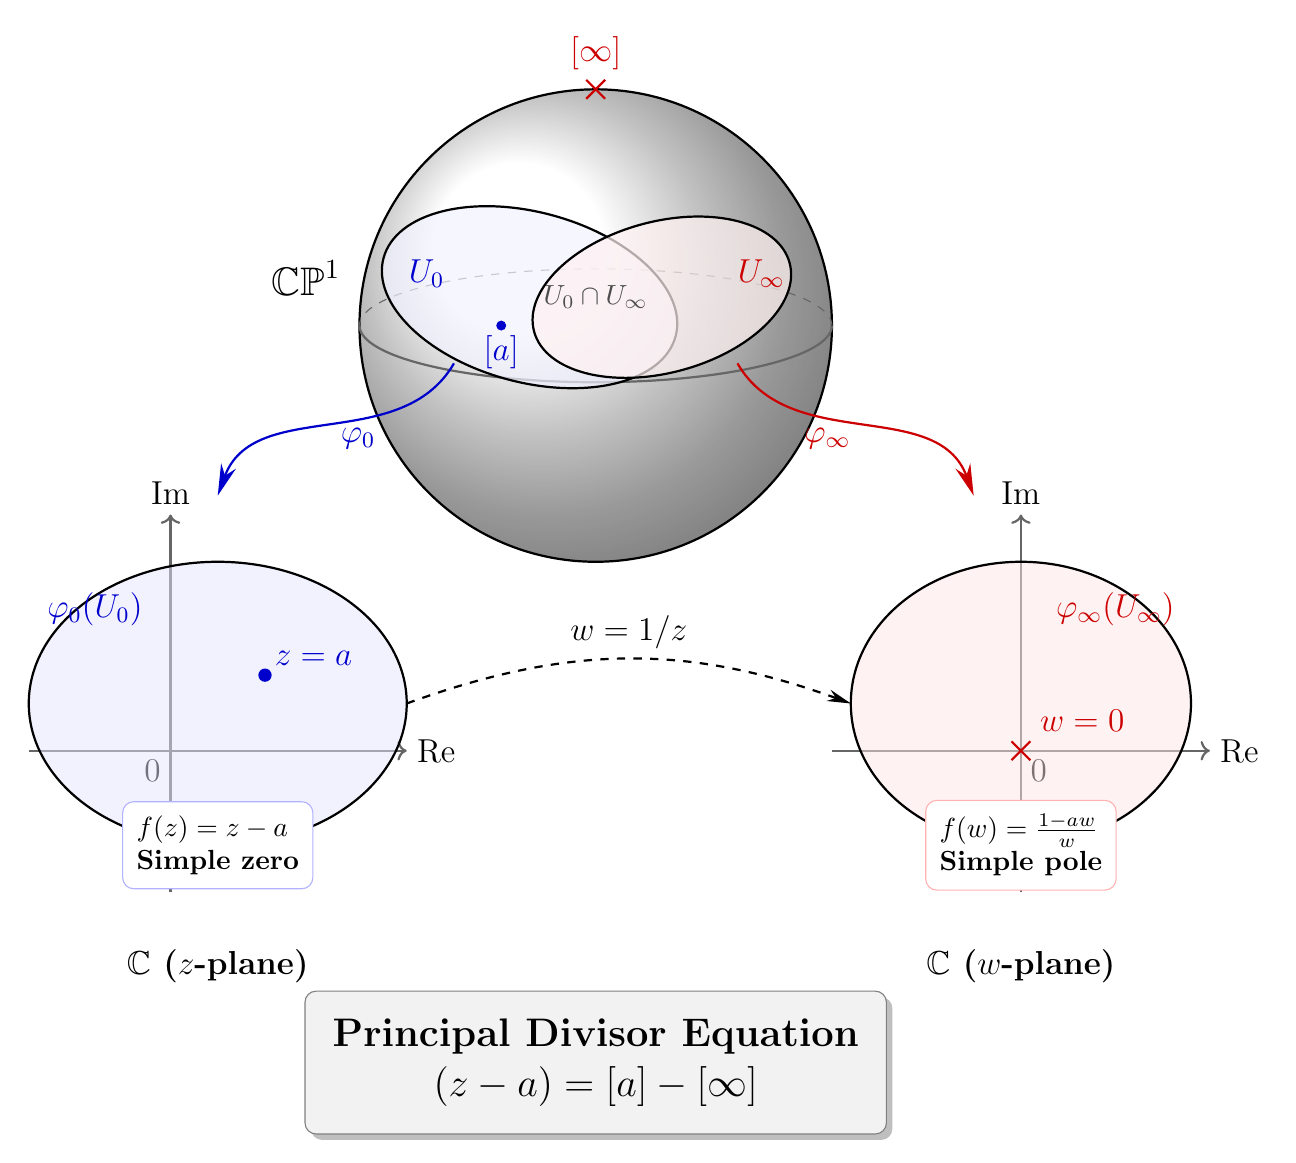
\begin{tikzpicture}[scale=1.2, every node/.style={font=\large}]
		
		% ==========================================
		% THE MANIFOLD (Riemann Sphere CP^1)
		% ==========================================
		% Sphere outline and 3D shading
		\shade[ball color=white, opacity=0.8] (0, 4) circle (2.5cm);
		\draw[thick] (0, 4) circle (2.5cm);
		
		% Equator for 3D perspective
		\draw[dashed, black!60] (2.5, 4) arc (0:180:2.5cm and 0.6cm);
		\draw[thick, black!60] (2.5, 4) arc (0:-180:2.5cm and 0.6cm);
		\node[left, font=\Large] at (-2.6, 4.5) {$\mathbb{CP}^1$};
		
		% Patch U_0
		\draw[thick, fill=blue!5, fill opacity=0.7, rotate around={-15:(-0.7, 4.3)}] 
		(-0.7, 4.3) ellipse (1.6cm and 0.9cm);
		\node[above left, blue!80!black] at (-1.5, 4.3) {$U_0$};
		
		% Point [a] (Zero)
		\fill[blue!80!black] (-1.0, 4.0) circle (1.5pt) node[below] {$[a]$};
		
		% Patch U_\infty
		\draw[thick, fill=red!5, fill opacity=0.7, rotate around={15:(0.7, 4.3)}] 
		(0.7, 4.3) ellipse (1.4cm and 0.8cm);
		\node[above right, red!80!black] at (1.4, 4.3) {$U_\infty$};
		
		% Point [\infty] (Pole at North Pole)
		\draw[red!80!black, thick] (-0.1, 6.4) -- (0.1, 6.6);
		\draw[red!80!black, thick] (-0.1, 6.6) -- (0.1, 6.4);
		\node[red!80!black, above] at (0, 6.6) {$[\infty]$};
		
		% Label the overlap conceptually
		\node[font=\normalsize, text=black!70] at (0, 4.3) {$U_0 \cap U_\infty$};
		
		% ==========================================
		% LOCAL COORDINATE CHARTS (Complex Planes)
		% ==========================================
		
		% --- Left Chart (z-plane on U_0) ---
		\begin{scope}[shift={(-4.5, -0.5)}]
			% Axes
			\draw[thick, ->, black!60] (-1.5, 0) -- (2.5, 0) node[right, text=black] {Re};
			\draw[thick, ->, black!60] (0, -1.5) -- (0, 2.5) node[above, text=black] {Im};
			\node[below left] at (0,0) {$0$};
			\node[below, font=\large\bfseries] at (0.5, -2.0) {$\mathbb{C}$ ($z$-plane)};
			
			% Image of U_0
			\draw[thick, fill=blue!10, fill opacity=0.5] (0.5, 0.5) ellipse (2cm and 1.5cm);
			\node[blue!80!black] at (-0.8, 1.5) {$\varphi_0(U_0)$};
			
			% Zero at a
			\fill[blue!80!black] (1.0, 0.8) circle (2pt) node[above right] {$z=a$};
			
			% Function Annotation
			\node[align=left, fill=white, draw=blue!30, rounded corners, inner sep=5pt, font=\normalsize] at (0.5, -1.0) {
				$f(z) = z-a$\\
				\textbf{Simple zero}
			};
			
			\coordinate (LeftOverlapAnchor) at (2.5, 0.5);
		\end{scope}
		
		% --- Right Chart (w-plane on U_\infty) ---
		\begin{scope}[shift={(4.5, -0.5)}]
			% Axes
			\draw[thick, ->, black!60] (-2.0, 0) -- (2.0, 0) node[right, text=black] {Re};
			\draw[thick, ->, black!60] (0, -1.5) -- (0, 2.5) node[above, text=black] {Im};
			\node[below right] at (0,0) {$0$};
			\node[below, font=\large\bfseries] at (0, -2.0) {$\mathbb{C}$ ($w$-plane)};
			
			% Image of U_\infty
			\draw[thick, fill=red!10, fill opacity=0.5] (0, 0.5) ellipse (1.8cm and 1.5cm);
			\node[red!80!black] at (1.0, 1.5) {$\varphi_\infty(U_\infty)$};
			
			% Pole at 0 (mapped from infinity)
			\draw[red!80!black, thick] (-0.1, -0.1) -- (0.1, 0.1);
			\draw[red!80!black, thick] (-0.1, 0.1) -- (0.1, -0.1);
			\node[red!80!black, above right] at (0.1, 0.1) {$w=0$};
			
			% Function Annotation
			\node[align=left, fill=white, draw=red!30, rounded corners, inner sep=5pt, font=\normalsize] at (0, -1.0) {
				$f(w) = \frac{1-aw}{w}$\\
				\textbf{Simple pole}
			};
			
			\coordinate (RightOverlapAnchor) at (-1.8, 0.5);
		\end{scope}
		
		% ==========================================
		% MAPPING ARROWS
		% ==========================================
		
		% \varphi_0 arrow
		\draw[-{Stealth[length=4mm, width=2mm]}, thick, blue!80!black] (-1.5, 3.6) to[out=-120, in=70] (-4.0, 2.2);
		\node[right, blue!80!black] at (-2.8, 2.8) {$\varphi_0$};
		
		% \varphi_\infty arrow
		\draw[-{Stealth[length=4mm, width=2mm]}, thick, red!80!black] (1.5, 3.6) to[out=-60, in=110] (4.0, 2.2);
		\node[left, red!80!black] at (2.8, 2.8) {$\varphi_\infty$};
		
		% Transition Map Arrow
		\draw[-{Stealth[length=3mm, width=1.5mm]}, thick, dashed] (LeftOverlapAnchor) to[bend left=20] node[above, font=\large] {$w = 1/z$} (RightOverlapAnchor);
		
		% ==========================================
		% DIVISOR CONCLUSION BOX
		% ==========================================
		\node[draw=black!50, fill=black!5, rounded corners, inner sep=10pt, align=center, drop shadow, font=\Large] at (0, -3.8) {
			\textbf{Principal Divisor Equation}\\
			$(z-a) = [a] - [\infty]$
		};
		
	\end{tikzpicture}
\end{document}